
\documentclass{sig-alternate-05-2015}

\usepackage{cite}
\begin{document}

% Copyright
\setcopyright{acmcopyright}
%\setcopyright{acmlicensed}
%\setcopyright{rightsretained}
%\setcopyright{usgov}
%\setcopyright{usgovmixed}
%\setcopyright{cagov}
%\setcopyright{cagovmixed}


% DOI
\doi{10.475/123_4}

% ISBN
\isbn{123-4567-24-567/08/06}

%Conference
\conferenceinfo{PLDI '13}{June 16--19, 2013, Seattle, WA, USA}

\acmPrice{\$15.00}

%
% --- Author Metadata here ---
\conferenceinfo{ASIA CCS}{'17  Abu Dhabi, UAE}
%\CopyrightYear{2007} % Allows default copyright year (20XX) to be over-ridden - IF NEED BE.
%\crdata{0-12345-67-8/90/01}  % Allows default copyright data (0-89791-88-6/97/05) to be over-ridden - IF NEED BE.
% --- End of Author Metadata ---

\title{Secure data Discovery and dissemination based on {short-length} public key scheme in Wireless sensor networks  }
%\subtitle{[Extended Abstract]
%\titlenote{}}
%
% You need the command \numberofauthors to handle the 'placement
% and alignment' of the authors beneath the title.
%
% For aesthetic reasons, we recommend 'three authors at a time'
% i.e. three 'name/affiliation blocks' be placed beneath the title.
%
% NOTE: You are NOT restricted in how many 'rows' of
% "name/affiliations" may appear. We just ask that you restrict
% the number of 'columns' to three.
%
% Because of the available 'opening page real-estate'
% we ask you to refrain from putting more than six authors
% (two rows with three columns) beneath the article title.
% More than six makes the first-page appear very cluttered indeed.
%
% Use the \alignauthor commands to handle the names
% and affiliations for an 'aesthetic maximum' of six authors.
% Add names, affiliations, addresses for
% the seventh etc. author(s) as the argument for the
% \additionalauthors command.
% These 'additional authors' will be output/set for you
% without further effort on your part as the last section in
% the body of your article BEFORE References or any Appendices.

\numberofauthors{2} %  in this sample file, there are a *total*
% of EIGHT authors. SIX appear on the 'first-page' (for formatting
% reasons) and the remaining two appear in the \additionalauthors section.
%
\author{
% You can go ahead and credit any number of authors here,
% e.g. one 'row of three' or two rows (consisting of one row of three
% and a second row of one, two or three).
%
% The command \alignauthor (no curly braces needed) should
% precede each author name, affiliation/snail-mail address and
% e-mail address. Additionally, tag each line of
% affiliation/address with \affaddr, and tag the
% e-mail address with \email.
%
% 1st. author
\alignauthor
Yan Wang\\
       \affaddr{East China Normal University}\\
       \affaddr{No.3663,Zhongshanbei Road}\\
       \affaddr{Putuo District,Shanghai,China}\\
       \email{boliangzai@foxmail.com}
% 2nd. author
\alignauthor
Daojing he\\
       \affaddr{East China Normal University}\\
       \affaddr{No.3663,Zhongshanbei Road}\\
       \affaddr{Putuo District,Shanghai,China}\\
       \email{djhe@sei.ecnu.edu.cn}
}
% There's nothing stopping you putting the seventh, eighth, etc.
% author on the opening page (as the 'third row') but we ask,
% for aesthetic reasons that you place these 'additional authors'
% in the \additional authors block, viz.

% Just remember to make sure that the TOTAL number of authors
% is the number that will appear on the first page PLUS the
% number that will appear in the \additionalauthors section.

\maketitle
\begin{abstract}

In Wireless Sensor Networks, WSNs, dissemination is typically used to query nodes, send commands, and reconfigure the network. In fact, WSNs are always deployed in harsh and open environment, it is important to judge messages as if they are from trusted source. Authentication can be satisfied by Public Key Cryptography (PKC). But PKC operations are expensive in terms of bandwidth, computing and storage consumption. To reduce costs, we propose a lightweight and Dos-resilient broadcast authentication mechanism using short-length public/private keys and presents its application in securing Drip protocol, an open source message dissemination protocol. We compare our mechanism with traditional 160-bit ECC public-key schemes, and show that our scheme can achieve a significant improvement on energy consumptions. Besides, we believe that our mechanism is able to fulfill the broadcast authentication requirements of WSNs.

\end{abstract}


%
% The code below should be generated by the tool at
% http://dl.acm.org/ccs.cfm
% Please copy and paste the code instead of the example below. 
%
\begin{CCSXML}
<ccs2012>
 <concept>
  <concept_id>10010520.10010553.10010562</concept_id>
  <concept_desc>Computer systems organization~Embedded systems</concept_desc>
  <concept_significance>500</concept_significance>
 </concept>
 <concept>
  <concept_id>10010520.10010575.10010755</concept_id>
  <concept_desc>Computer systems organization~Redundancy</concept_desc>
  <concept_significance>300</concept_significance>
 </concept>
 <concept>
  <concept_id>10010520.10010553.10010554</concept_id>
  <concept_desc>Computer systems organization~Robotics</concept_desc>
  <concept_significance>100</concept_significance>
 </concept>
 <concept>
  <concept_id>10003033.10003083.10003095</concept_id>
  <concept_desc>Networks~Network reliability</concept_desc>
  <concept_significance>100</concept_significance>
 </concept>
</ccs2012>  
\end{CCSXML}
%
\ccsdesc[500]{Computer systems organization ~ WSNs}


\ccsdesc[300]{
Cryptography~ Public key}

%

%
% End generated code
%

%
%  Use this command to print the description
%
\printccsdesc

% We no longer use \terms command
%\terms{Theory}

\keywords{Public key; message dissemination, Dos resilience}

\section{Introduction}
Wireless sensor networks are being used in a wide variety of applications, such as military sensing and tracking, industrial control. Sensor networks are composed of one or more base stations and a number of sensor nodes. Obviously, wireless industrial control sensor networks are broadcast networks and channels are shared among all users in the network. 

As shown in Fig.1, when deployed in hostile environments, sensor networks are susceptible to a variety of attacks. For example, adversaries are able to easily intercept the messages between base stations and sensor nodes, impersonate the base stations to deceive sensor nodes. 

Many countermeasures such as PKC, have been developed to prevent adversaries from impersonating base stations. But these countermeasures make sensor networks an easy target of Dos attacks. We provide an example to illustrate this problem. 

First, as shown in Fig.1, sensors are measuring temperature, the control center may want sensors to measure humidity of the atmosphere instead. In this case, control center need broadcast values to reconfigure the whole network. 
In mentioned network, communications are based on IEEE 802.11.4 standard. It is open and adversaries can broadcast a large number of bogus messages, exhausting resources of sensor nodes.

\begin{figure}
\centering
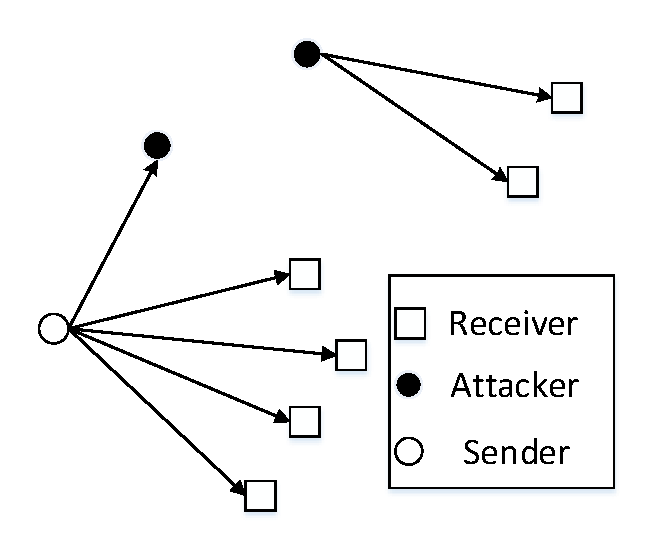
\includegraphics[width=5cm,height=4cm]{Attack_scenario.pdf}\\
\caption{Attack scenario}\label{} 
\end{figure}

In order to secure message broadcast in industry control sensor networks.
This paper has the following major contributions:
\begin{itemize}
\item[1] First, We study the specific requirements needed to secure a WSNs protocol. According to security weaknesses and efficiency problem, we 
review existing broadcast authentication mechanisms.
\item[2] We propose a secure, lightweight, robust, Dos-resilient authentication mechanism. It is a secure extension of Drip and has advantages over traditional broadcast authentication protocol. 
\item[3] We conduct extensive experiments with many telosb platforms. And experimental data in chart shows that our mechanism can achieve high efficiency and performance.
\end{itemize}

\textbf{Organization} The organization of our paper is as follows:  Section II, we discuss the related work as the context of our work, and Section III describes the network model, security requirements and assumption. In Section IV, We present our scheme in detail. Section V analyses the security and efficiency properties of our protocol. Section VI describes the implementation and experimental results of the proposed protocol via real sensor platforms. Finally, Section VII concludes this paper. 

\section{Relate1d Work}
\subsection{Existing Work on Broadcast Authentication}
There are many challenges in information security protection of Wireless Sensor Networks. The primary one is the limited computing, communication and storage capabilities of a sensor node. Based on this factor, a number of broadcast authentication schemes, including symmetric key scheme and asymmetric key schemes, have been proposed, . 

A MAC algorithm, sometimes called a keyed hash function, outputs a tag derived by accepting a secret key and an arbitrary-length message as input\cite{TinySec}. The MAC value protects both a message's data integrity as well as its authenticity, by allowing verifiers who also possess the secret key to detect any changes to the message content.

But it is not desirable for broadcast authentication. Since key is shared among senders and receivers, any one of receivers can impersonate sender and forge messages using key.

Along with the development of related technology, asymmetric key schemes become more and more practical in wireless sensor network. 

Public key cryptography, or asymmetric cryptography, is a cryptographic system that uses pairs of keys: public keys which may be disseminated widely, and private keys which are known only to the owner. This typically achieve authentication function when the public key is used to verify identity of the message sender. Because of high computation costs and large signature size, public key cryptography in WSNs is susceptible to Dos attack. That is, the adversary may flood a large number of illegal signature messages to exhaust receivers' resources and render them less capable of serving legitimate users. 

In order to solve above problems, some researchers proposed TESLA\cite{Tesla} and its various extensions \cite{multi} to authenticate broadcast packets in a network.

TESLA is an example protocol in which authentication information is sent post the broadcast message. It employs symmetric cryptographic technique with delayed key disclosure, i.e., the key used to authenticate a message is disclosed in next message. However, time synchronization is required between sender and receiver. \cite{Tesla} have used a direct time synchronization between sender and receiver. Due to delayed key disclosure, TESLA protocol is susceptible to Dos attack.

If adversary sends a huge number of useless packets, it will take sensor nodes large memory space to store these packets until sensor nodes receive authentication key.

Other authentication schemes use one-time signature\cite{Biba},\cite{HORSIC}. Verification and authentication based on one time signature is very fast. Unfortunately, such schemes suffer from large key sizes and a limited number of uses per key.

To reduce cost, authors in \cite{aspect}, \cite{aspect} use a single signature to authenticate multiple data packets. In \cite{aspect}, sender have already known messages in advance and applied hash function to the last message, and output a hash value. Then sender attach this value to the previous message. This process is continued until the first message. Then sender just sign the first message using private key. Thus sender get a signature on all messages to be disseminated. After the first message is verified, the hash value of next message is also verified. We just use this hash value to authenticate next message. And recursively, the last message will be verified through its previous packet. Obviously, this protocol does not adapt to the changing environment, WSNs needs administrator to configure the network frequently, we cannot predict next message to be sent. 


Another approach has been adopted by some researchers \cite{hashtree}, who use a Merkle tree instead of recursive hashing for packet authentication. This approach require to include many hash value in a packet, increasing bandwidth consumption.

Also, hash chain approach \cite{nested} is a method to verify packet. But its high performance requires good network communication channel. Once wireless network is affected severely, the authentication process behind the lost packet is not able to continue.
 
\subsection{Review on Message Dissemination}
Drip is one of the most popular message dissemination protocol in sensor networks. In Drip, each message is represented as a 3-tuple (key, seqno, data), where key uniquely identifies the variable to be updated, data denotes the disseminated data item (e.g., parameter, command or query), and seqno indicates if the data item is old or new (the larger the seqno, the newer the data). In the Drip implementation, key and seqno are 2 bytes and 4 bytes long, respectively. Drip disseminates each data item with a separate instance of Trickle algorithm \cite{trickle}. Once new data are injected to a receiver by the sender, they will be disseminated by Trickle quickly.

With Trickle algorithm, the problem of packet loss are greatly improved. Since the goal of a dissemination protocol is to reliably deliver a piece of data to every node in the network.
	
	Although we have used Drip for our reference implementation, our mechanism can be extended to other popular broadcast protocols, with the assumptions listed in Section III.C. In the rest of this paper, unless otherwise specified, we assume that Drip is used as the message dissemination protocol

\section{ PROBLEM DEFINITION}
\subsection{Network Model}
	We consider a broadcast network consists of one sender (\emph{S}) and a group of receivers (\emph{R$_i$}). Each message is delivered from S to every \emph{R$_i$} through lossy and insecure network, as illustrated in Fig. 2. The intermediate receivers in the network only forward the packets and do not provide any security measures (such as integrity and authenticity checks). These receivers may be malicious to drop or modify \emph{S}$'$s packets or even inject fake packets.
	
	We consider a class of applications where
	
	1) each generated message is unknown to \emph{S} until it is ready to send; 
	
	2) \emph{S} (resp.\emph{R}) signs (resp. verifies) the message once it appears; 
	
	3) the sending rate at \emph{S} is dynamic. And the data flow of the broadcast authentication protocol is shown in Fig. 5
	
	
\begin{figure}
\centering
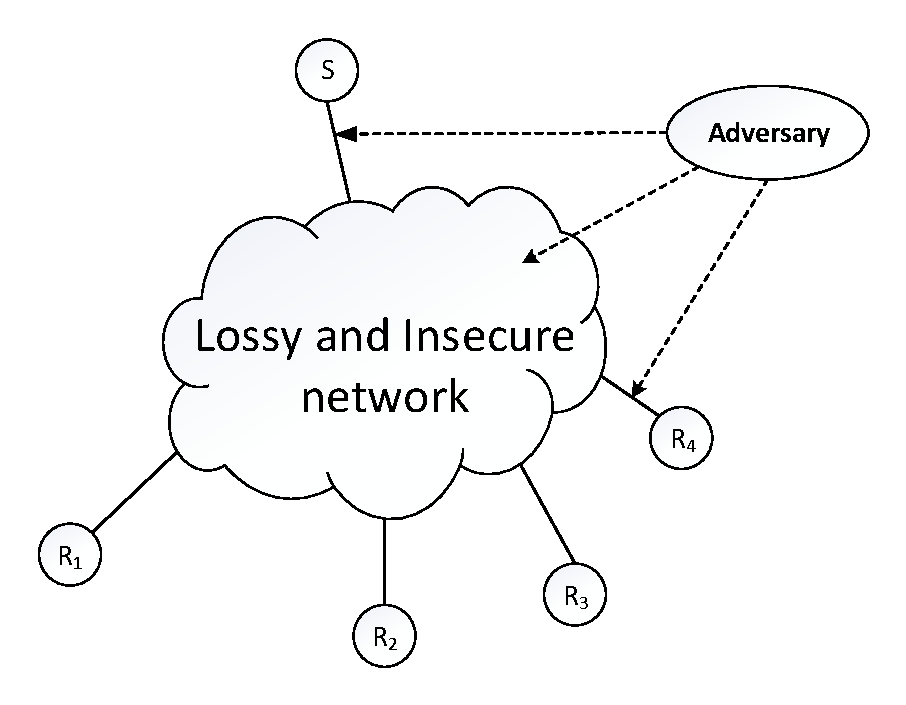
\includegraphics[width=6cm,height=4cm]{NetworkModel.pdf}\\
\caption{Network Model}\label{} 
\end{figure}

\subsection{Requirement}
In addition to the asymmetric mechanism that is needed for broadcast authentication, an efficient and secure broadcast authentication scheme for Wireless Sensor Networks should still satisfy the following requirements:

\begin{itemize}
\item[1] Individual authentication: The receiver should verify the received packets individually without depending on other packets; otherwise, the failure to verify a packet prevents the verification of subsequent packets.

\item[2] Robust to packet loss: The smart grid communication environment is not reliable; therefore, the scheme should be able to cope with the loss of packets during trans- mission.

\item[3] Short authentication latency: Many PLC applications are real time applications, e.g. sending the control informa- tion to the customers. To authenticate real time data, the maximum number of additional packets that need to be received before a packet can be authenticated should be small.

\item[4] Low computation cost: Receivers have limited compu- tation power. Thus, they should only perform a small number of operations to verify a packet.

\item[5] Receiver compromise tolerance: The protocol should be resilient to receiver compromise attack no matter how many receivers have been compromised, as long as the subset of non-compromised receivers can still form a connected graph with the trusted source.

\item[6] Low communication overhead: Because a PLC network often is restricted in bandwidth, the number of bytes per packet used for authentication should be small.

\item[7] DoS attacks resistance: The functions of the PLC net- work should not be disrupted by DoS attacks.

\item[8] Freshness: A receiver should be able to differentiate whether an incoming message is the newest version.

\item[9] Scalability: The protocol should be efficient even for large-scale smart grids with thousands of receivers.

\item[10] Low storage requirement: Since the storage space of receivers is limited, some data for authentication like key material and signatures stored in memory cannot be too large.
\end{itemize}

\begin{figure}
\centering
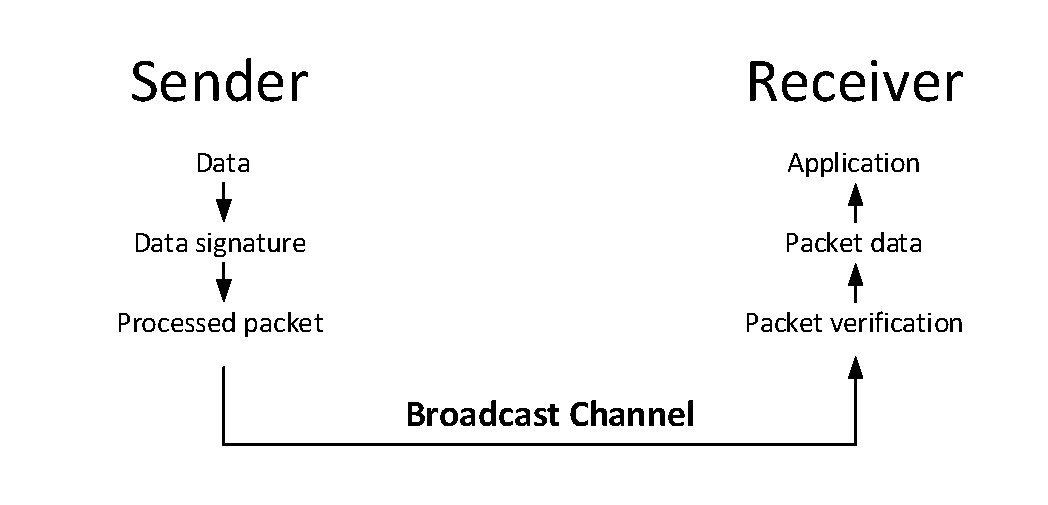
\includegraphics[width=8cm,height=4cm]{DataFlow.pdf}\\
\caption{DataFlow}\label{} 
\end{figure}

Ideally, we would like a scheme that is able to recover from any loss of packets, has no authentication latency, can individually authenticate packets and ensure data confidentiality, has negligible overhead, and has a low computation cost. In practice, such a perfect scheme is difficult to achieve, and a compromise needs to be found between these requirements.
\subsection{Assumption}
Our protocol makes the following assumption.
\begin{itemize}
    \item The sender cannot be compromised, and is trusted. In Drip, the sender is the origin of all legitimate message updates. The sender has unlimited computational power compared with receiver.
    \item  The receiver can perform a limited number of asymmetric cryptographic operations such as signature verification in TinyECC [15], but they cannot afford to perform many such operations due to their energy limitations.
\end{itemize}
\section{The Proposed Protocol}
Before giving the detailed description of the proposed protocol, we first provide an overview of our protocol.
\subsection{Overview of Our Protocol}
Elliptic curve cryptography is an outstanding approach to public-key cryptography in terms of strength. Traditionally, the cost of public key operations may dominate the cost of transmitting packets in sensor network. Since broadcast authentication requires sensors to conduct a large number of PKC operations, using PKC in the traditional way is still impractical. It is desirable if we can significantly reduce the cost of PKC operations by optimizing the broadcast authentication protocols.
We propose ShortPK approach, i.e. short-length public key, for example, if we reduce an ECC public key from 160bits to 80 bits, the computation cost for signature is reduced to roughly one eighth and the length of signatures is reduced to half. While short-length public key is easy to break, we need a more efficient way to distribute short-length public keys. With enough memory, we can load public keys into sensor$'$s memories before sensor deployment. But the public keys must be encrypted, otherwise one sensor is compromised, the public keys will be compromised.  We can use AES for the symmetric-key encryption, therefore nobody, including sensor nodes, knows public keys before the arrival of decryption key included in broadcast packet. 

Meanwhile, we denote encryption key as \emph{K$_i$}, i means the \emph{i-th} dissemination. However, it is important that sensor nodes are able to verify \emph{K$_i$} in each of the broadcast packet. If the adversary randomly chooses a key \emph{K$_i '$} and a public key \emph{PK$_i '$} , encrypts \emph{PK$_i '$} into (\emph{PK$_i '$})\emph{K$_i '$} using \emph{K$_i '$}, both \emph{PK$_i '$} and \emph{K$_i '$} are invalid. When receiving packet, sensors do not verify \emph{K$_i$}, then will get a gibberish \emph{PK$_i '$}. They will use \emph{PK$_i '$} as the public key to conduct signature verification. Even though the verification is not successful, sensors spend a lot of energy and time verifying the signature.

Therefore, sensors need to verify whether the received \emph{K$_i '$} is from the basestation or not. This can be achieved by one-way hash chain.

\begin{figure}
\centering
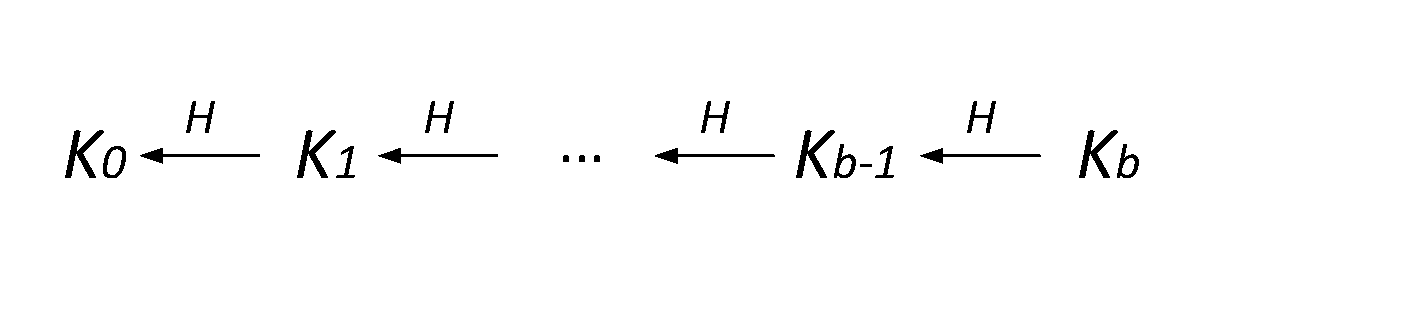
\includegraphics[width=10cm,height=2cm]{HashChain.pdf}\\
\caption{Hash Chain}\label{} 
\end{figure}

As illustrated in Fig.4, the sender randomly chooses a number \emph{K$_b$}, and then generates a one-way hash chain. A hash chain is based upon a public function \emph{H} that is easy to compute, but computationally difficult to invert -- thus, the term, one-way hash chain. A hash chain of length \emph{b} is generated by repeatedly applying the hash function \emph{H} to the last element, say, \emph{K$_b$}, in the chain, to generate a sequence of hashes such that \emph{K$_j$} = \emph{H}(\emph{K$_{j+1}$}). The head of the chain, \emph{K$_0$}, serves as a commitment to the entire hash chain. The hash chain is generated in the order \emph{K$_b$},\emph{K$_{b-1}$}, ..., \emph{K$_1$}, \emph{K$_0$} and revealed in the reverse order. Here \emph{b} is the maximum number of message disseminations permitted in the lifetime of the WSNs. The keys \emph{K$_0$}, \emph{K$_1$}, ...,\emph{K$_b$} are referred to as puzzle keys, and \emph{K$_j$} is used for the \emph{j-th} disseminated messages, where \emph{j}> 0.

% Hash Chain element  %

But adversaries can intercept the communication channel between base station and sensor nodes. The encryption key broadcasted in open channel is exposed to adversaries. By compromising sensor nodes, the cipher text of \emph{PK$_i '$} is also obtained by adversary. Based on mentioned information, adversary is able to get public key by decrypting cipher text stored on sensor nodes using intercepted key. After getting Public key, adversary is able to forge a malicious packet containing \emph{data}$'$, that is (\emph{data}$'$), \emph{K$_i$}, \emph{signature}. \emph{signature} is produced using decrypted public key.
		
		Obviously, it take adversary time to listen to communication in channel and forge a malicious packet. 
		We must prolong the time for adversary to produce an invalid packet. Here we can use message specific puzzle, make the packet hard to produce. That is, without solving a message specific puzzle first, adversary cannot send a malicious packet.

\subsection{System Initialization Phase}
In this stage, the sender sets up an ECC by deriving a private key SK and public parameters {PK,Q, p, q,H(.)} by performing the following operations. It selects an elliptic curve E over GF(p), where p is a big prime number. Here Q denotes the base point of E while q is also a big prime number and  represents the order of Q. It then picks the private key SK $\in$ GF(q) and generates the public key PK = SK$\cdot$Q. As an illustrative example, for 160-bit ECC, both PK and Q are 320 bits long, and both p and q are 160 bits long.

Using a node of one-way hash chain as security key, strong encryption is achieved through the use of a 128-bit AES algorithm. The cipher text is loaded on every sensor nodes, thus adversary is not able to squeeze any key information out of cipher text. On the basis of AES algorithm, we can use small-sized public key and small-sized signature to keep our protocol cost-effective. 

The secret key is included in broadcast packet.     

If the public keys are not encrypted, adversaries can immediately get all the public keys, and will have much longer enough time to find the corresponding private keys.

In this stage, sender transforms public keys into ciphertext, (\emph{PK$_i$})\emph{K$_i$}. The encryption keys, denoted as \emph{K$_1$},,,\emph{K$_N$}, are the elements of hash chain in Fig.1. \emph{K$_i$} is the \emph{i-th} key in the one-way key chain.  

The committed value of this hash chain (i.e., \emph{K$_0$}) and ciphertext of public keys (\emph{PK$_i$})\emph{K$_i$} are preloaded in each receiver of the network before deployment, together with the public parameters {PK, Q, p, q,H(.)} of the sender. Any of the reported secure key pre-distribution schemes (e.g., [16], [17]) may be used for this purpose. The hash chain is called the version chain as its elements correspond to update versions of the message. The \emph{j-th} element of this hash chain stored in the sensor receiver is called \emph{j-th} version key.

\subsection{Pakcet Pre-processing Phase}
Our solution is keyed message-specific puzzles based on one-way key chains
(or briefly, message-specific puzzles). Intuitively, to prevent an attacker from precomputing puzzle solutions to forged messages, we add in such a puzzle a previously undisclosed key in the one-way key chain. As a result, an attacker cannot precompute a puzzle solution until such a key is released by the sender. Upon receiving such a packet, any node can easily verify the puzzle solution. However, we develop the puzzle system in such a way that it will take a substantial amount of time to solve such a puzzle. As a result, even if the key \emph{K$_i$} is released in a broadcast packet, an attacker cannot immediately solve the puzzle for a forged packet, and thus cannot immediately launch Dos attacks.

Now let us describe the details of message specific puzzles. As in the strawnman approach, we assume the sender has generated a one-way key chain consisting of  \emph{K$_0$} \emph{K$_1$} ... \emph{K$_n$}, and distributed \emph{K$_0$} to all potential receivers. 

		Given the \emph{i-th} message M$_i$, the sender first generates the broadcast authenticator, i.e., signature$_i$, and K$_i$ then construct the puzzle, which we call the i-th message specific puzzle. For the sake of presentation, we denodte the solution to this puzzle as P$_i$. As shown int Figure.5.
		
	

A valid solution P$_i$ to the i-th message-specific puzzle, where 1 $\leq$ i $\leq$n, must satisfy the following condition:
After applying the hash function Fp to the i-th message-specific puzzle and its solution, we get an image where the first l bits are all ``0''. That is,
F(i | Mi | signature | Ki | P) = 0000xxxxxx
where ``xxx..'' represents any bit pattern. The parameter l is called the strength of the puzzle.
Because of the one-way property of the hash function Fq, one has to search through the space of possible solutions to solve the puzzle. In other words, given Mi signature Ki for each candidate solution W, the sender (or an attacker) has to verify if the first l bits of Fp(Mi, signature, Ki p) are all ``0''.
Finally, the sender then broadcasts the packet with the payload i | Mi | signature | Ki | P .
		
\begin{figure}
\centering
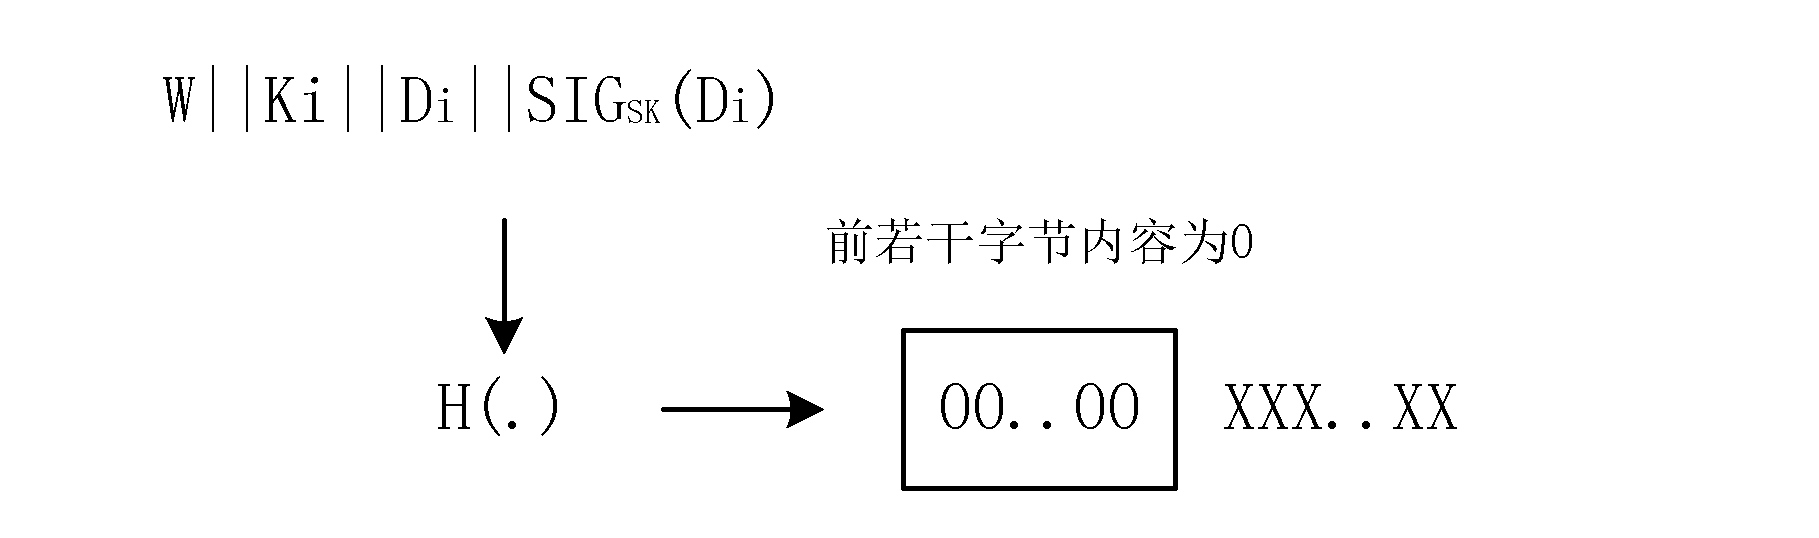
\includegraphics[width=8cm,height=2cm]{SpecificPuzzle.pdf}
\caption{specific puzzle}
\label{} 
\end{figure}



\subsection{packet verification phase}
Upon receiving a broadcast packet, each receiver first verifies the puzzle solution, If the puzzle solution is invalid, the receiver will simply drop this packet. 

Then receiver verifies the puzzle key K1 included in the packet, i.e., whether the hash result of K1 equals to K0 or not.

If the puzzle key k1 is authentic, we can use it to decrypt the ciphertext stored in receiver nodes. 
After that, signature included in packet will be verified by decrypted public keys. 

Then, receiver accept the data included in packet.
\section{Security And Efficiency Analysis}
\subsection{Security Analysis}
\textbf{Integrity of Data Items}
In our protocol, the base station is trustworthy. It signs every message with the generated private key. Since private key is only known to base station,  receivers are able to authenticate the identity of message's sender.  On the basis of signature, receiver can verify the data upon receiving them.

\textbf{Resistance to Dos Attacks}
As discussed in related work, there are three types of Dos attacks against basic our protocol:
\begin{enumerate}
\item Dos attacks exploiting authenticatio delays.
\item Dos attacks exploiting the expensive signature verifications, and 
\item Dos attacks exploiting Trickle algorithm.
\end{enumerate}

Ourprotocol is resistant to all three types Dos attacks. Due to the use of message specific puzzle, upon receiving a packet, each node can verify it immediately through performing efficient hash function. Further, because of short-length public key, the verification does not take long time.

 Without passage of key verification, anyone cannot misuse trickle algorithm.
 
   Adopting our protocol, WSNs is immune to all three types of Dos attacks. Indeed, without enough time and private key, attackers is not able to paralyze WSNs through  producing a valicious packet or falsifing valid message.
   
\textbf{Efficiency Analysis}   
    Only if the verification of the puzzle included in the signature packet is successful will each node execute the signature verification operation.
	While being transmitted, short-length signature consumes  little bandwidth. It is fast hash  function that verifies a specific puzzle. Hash function is fast and efficient on sensor node.
	Thus our protocol requires little computing overhead . Also sensor nodes spend only a little amount of memory to store public keys.
	

\section{Implementation And Performance Evaluation}
We evaluate our protocol by implementing all its components in an experimental test-bed. Also, we choose Drip for performance comparison.

\subsection{Implementation and Experimental Setup}
Our implementation has the base station and sensor node side programs. The base station side programs are C programs using OpenSSL. All programs and application on base station side is running on virtual machine, VMware Workstation, which is a distinguished software. Besides, the sensor node side programs are written in nesC, a event-driven programming language. NesC is running on resource-limited  sensor motes, Telsob. The Telosb mote has an 8-MHz CPU, 10-kB RAM, 48-kB ROM, 1MB of flash memory, and an 802.15.4/Zigbee radio. Telosb, nesC, is specially designed for TinyOS, an open source operating system designed for wireless devices. 
The key size of ECC is set to 128 bits and SHA-1 is used. Without additional specification,
we repeated one million times (resp., one thousand times) for each measurement in order to obtain a objective accurate results.

To implement our protocol, we add the following functionalities in the C tools on the base station side: construction of specific puzzles. 

In the implementation of Drip, when a packet with a new version number is received, a node stores the packet and then resets the Trickle timer. In our protocol, when a packet with a new version number is received, a node stores the packet and then authenticates it. If the result is positive, the node resets Trickle timer; otherwise, the node simply discards the packet. In  an improved protocol, the packet additionally contains a specific puzzle, the result is different.

Following the design of our protocol described above, we employ the ECDSA verify and SHA-1 hash operations of TinyECC 2.0 library to add the verification function of signature packet into the Drip nesC library. 
In our implementation, the base station (i.e. a laptop PC) first sends the signature and data packets through a serial port to a particular sensor node which is referred to as disseminator. Then, the disseminator disseminates these packets by Drip.

Similar to , we have built a circuit as shown in Fig.4 to measure the power consumption in resource-limited sensor nodes when they execute various cryptographic .



\subsection{Evaluation Results}
Our implementation is very good.

\begin{figure}[ht]
\begin{center}
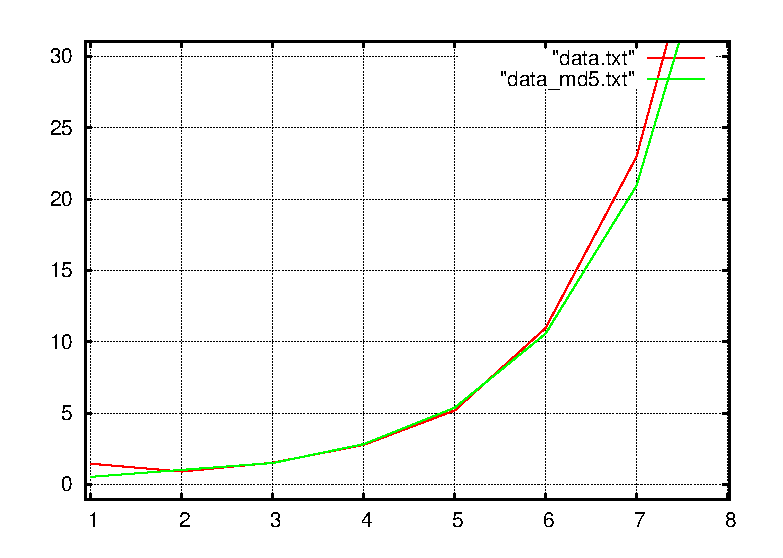
\includegraphics[width=8cm,height=5cm]{compare_color.eps}
\end{center}
\caption{DataFigure}\label{fig:SSDArchitecture}
\end{figure}

\begin{figure}[ht]
\begin{center}
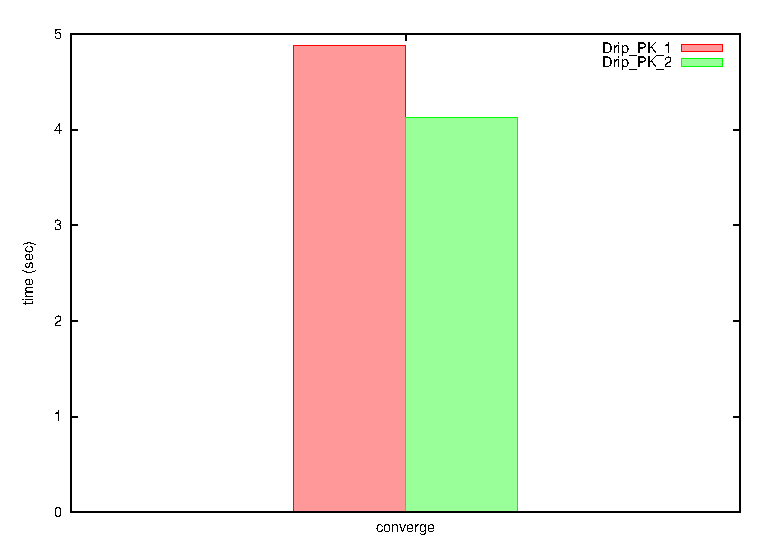
\includegraphics[width=8cm,height=5cm]{converge.eps}
\end{center}
\caption{DataFigure}\label{fig:SSDArchitecture}
\end{figure}


The charts in Fig.7 show the average times for each operation phase in TinyECC. This charts shows that ECC with secp128r1 has no advantage over that with secp160r1. It has the similar time consumption with secp160r1. But shortness is a virtue we appreciate in packet broadcast, which consumes major bandwidth and power of sensor node. Besides, in initiation phase, secp128r1 is the fastest. It will help quick deployment of WSNs under some exceptional circumstances.

\begin{figure}[ht]
\begin{center}
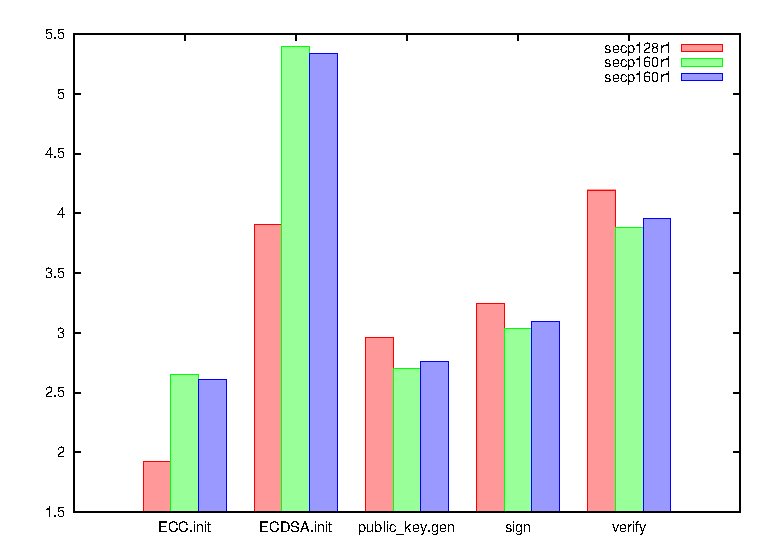
\includegraphics[width=8cm,height=5cm]{2.eps}
\end{center}
\caption{DataFigure}\label{fig:SSDArchitecture}
\end{figure}


\section{Conclusions}

In this paper, we have identified the security vulnerabilities in data discovery and dissemination of WSNs. We then developed a lightweight protocol  to allow efficient authentication of the disseminated data items by taking advantage of short-length public key. Our protocol is designed to work within the computation memory and energy limits of inexpensive sensor motes. In addition to analyzing the security of Our protocol, this paper has also reported the evaluation results of Our protocol in an experimental network of resource-limited sensor nodes, which show that our protocol is efficient and feasible in practice.


\section{Acknowledgments}

\bibliographystyle{abbrv}
\bibliography{sigproc}  % sigproc.bib is the name of the Bibliography in this case

\appendix
%Appendix A

\begin{thebibliography}{13}

\bibitem{TinySec} Karlof C, Sastry N, Wagner D. TinySec: a link layer security architecture for wireless sensor networks[C]//Proceedings of the 2nd international conference on Embedded networked sensor systems. ACM, 2004: 162-175.

\bibitem{Tesla} Perrig A, Canetti R, Tygar J D, et al. The TESLA broadcast authentication protocol[J]. RSA CryptoBytes, 2005, 5.

\bibitem{multi}Liu D, Ning P. Multilevel μTESLA: Broadcast authentication for distributed sensor networks[J]. ACM Transactions on Embedded Computing Systems (TECS), 2004, 3(4): 800-836.

\bibitem{proceeding1} Czajkowski, K., Fitzgerald, S., Foster, I., Kesselman, C.: Grid
Information Services for Distributed Resource Sharing. In: 10th IEEE
International Symposium on High Performance Distributed Computing, pp.
181--184. IEEE Press, New York (2001)

\bibitem{HORSIC} Lee J, Kim S, Cho Y, et al. HORSIC: An efficient one-time signature scheme for wireless sensor networks[J]. Information Processing Letters, 2012, 112(20): 783-787.

\bibitem{asurvey} Grover K, Lim A.: A survey of broadcast authentication schemes for wireless networks[J]. Ad Hoc Networks, 2015, 24: 288-316.

\bibitem{Biba} Perrig A.: The BiBa one-time signature and broadcast authentication protocol[C]//Proceedings of the 8th ACM conference on Computer and Communications Security. ACM, 2001: 28-37.

\bibitem{aspect} He D, Chan S C, Guizani M.: Small data dissemination for wireless sensor networks: The security aspect[J]. Wireless Communications, IEEE, 2014, 21(3): 110-116.

\bibitem{nested} Eldefrawy M H, Khan M K, Alghathbar K, et al. Broadcast authentication for wireless sensor networks using nested hashing and the Chinese remainder theorem[J]. Sensors, 2010, 10(9): 8683-8695.

\bibitem{hashtree}He D, Chan S, Tang S, et al. Secure data discovery and dissemination based on hash tree for wireless sensor networks[J]. IEEE transactions on wireless communications, 2013, 12(9): 4638-4646.

\bibitem{efficient} Perrig A, Canetti R, Tygar J D, et al.: Efficient authentication and signing of multicast streams over lossy channels[C]//Security and Privacy, 2000. IEEE Symposium on. IEEE, 2000: 56-73.%Here I delete S&P 2000

\bibitem{trickle}Patel N, Culler D, Shenker S.: Trickle: A self regulating algorithm for code propagation and maintenance in wireless sensor networks[M]. Computer Science Division, University of California, 2003.

\bibitem{lnicstchap} May, P., Ehrlich, H.C., Steinke, T.: ZIB Structure Prediction Pipeline:
Composing a Complex Biological Workflow through Web Services. In: Nagel,
W.E., Walter, W.V., Lehner, W. (eds.) Euro-Par 2006. LNCS, vol. 4128,
pp. 1148--1158. Springer, Heidelberg (2006)

\bibitem{proceeding2} Foster, I., Kesselman, C., Nick, J., Tuecke, S.: The Physiology of the
Grid: an Open Grid Services Architecture for Distributed Systems
Integration. Technical report, Global Grid Forum (2002)

\bibitem{url} National Center for Biotechnology Information, http://www.ncbi.nlm.nih.gov

\bibitem{Msp}He D, Chan S C, Tang S, et al. Secure Data Discovery and Dissemination based on Hash Tree for Wireless Sensor Networks[J]. IEEE Transactions on Wireless Communications, 2013, 12(9):4638-4646.
\end{thebibliography}
\end{document}
